\documentclass[brudnopis]{xmgr}
% Jeśli nowe rozdziały mają się zaczynać na stronach nieparzystych:
%\documentclass[openright]{xmgr}

% install minted package to highlight source code
% \usepackage{minted}
\usepackage{listings}
\lstset{language=Python}
\lstset{frame=lines}
%\lstset{caption={Insert code directly in your document}}
\lstset{label={lst:code_direct}}
\lstset{basicstyle=\footnotesize}
%\defaultfontfeatures{Scale=MatchLowercase}
%\setmainfont[Numbers=OldStyle,Ligatures=TeX]{Minion Pro}
%\setsansfont[Numbers=OldStyle,Ligatures=TeX]{Myriad Pro}
% for fontspec version < 2.0
% \setmainfont[Numbers=OldStyle,Mapping=tex-text]{Minion Pro}
% \setsansfont[Numbers=OldStyle,Mapping=tex-text]{Myriad Pro}
%\setmonofont[Scale=0.75]{Monaco}
\usepackage{marginnote}
% Opcjonalnie identyfikator dokumentu
% drukowany tylko z włączoną opcją 'brudnopis':
\wersja   {wersja wstępna [\ymdtoday]}

\author   {Adam Makiewicz}
\nralbumu {235281}
\email    {adammak23@gmail.com}


\title    {Generowanie płytek obwodu drukowanego w środowisku Python jako dodatek do programu graficznego Blender}
\date     {2020}
\miejsce  {Gdańsk}

\opiekun  {dr Piotr Arłukowicz}

% dodatkowe polecenia
%\renewcommand{\filename}[1]{\texttt{#1}}
%\definecolor{stress}{cmyk}{0,1,0.13,0} % RubineRed
%\definecolor{topic}{cmyk}{0.98,0.13,0,0.43} % MidnightBlue

\begin{document}

% TOOD: ZMIENIĆ STRESZCZENIE

%2 Kolejny rozdział przedstawi natomiast szczegóły implementacji każdego z przedstawionych elementów.
\begin{abstract}
Istnieje wiele programów do projektowania płytek drukowanych, jednak żadne z nich, z uwagi na swoje ścisłe zastosowania, nie posiadają odpowiednich narzędzi do zaawansowanego renderowania, animacji i tworzenia szeroko pojętej “sztuki”. Popularny program do tworzenia grafiki 3D - Blender, z uwagi na możliwość rozbudowania go o dodatki jest znakomitym narzędziem mogącym wspomagać ten proces.
\end{abstract}


% słowa kluczowe
\keywords{wizualizacja, grafika, 3D, Blender, Python, PCB, elektronika}

% tytuł i spis treści
\maketitle

% wstęp
\introduction

Obwody drukowane czy też inaczej płytki drukowane (zwane dalej "PCB", ang. Printed Circuit Board) to podstawa dla każdego modułu elektronicznego. Dzięki swojej budowie oraz dobranym częściom składowym pozwalają inżynierom z roku na rok konstruować coraz to nowocześniejsze i bardziej funkcjonalne urządzenia. PCB służy przede wszystkim do montowania wszelkich podzespołów elektronicznych oraz zapewnienia im wspólnego stabilnego połączenia.

Tworzenie PCB składa się z trzech głównych etapów: \cite{Abboud}

\begin{itemize}
\item
Logic Design - Stworzenie schematu logiki i reguł projektowych, spis użytych komponentów i ich wzajemnych połączeń
\item
Layout - Zaprojektowanie układu, który decyduje o fizycznym położeniu i połączeniach (tzw. trasowanie -- \emph{routing}) komponentów
\item
Produkcja przemysłowa
\end{itemize}
    
    Najważniejszym punktem projektowania układu jest rozmieszczenie komponentów. Ten proces jest satysfakcjonującym, twórczym przedsięwzięciem i prawdopodobnie jednym z najtrudniejszych aspektów procesu projektowania PCB. Wielu inżynierów uważa go za formę sztuki gdyż w przeciwieństwie do schematu, który opiera się tylko na matematyce, jest nieco bardziej płynny i elastyczny oraz pozwala na kreatywne wdrożenie swojego projektu w życie.

\begin{figure}[!tbh]
\centering
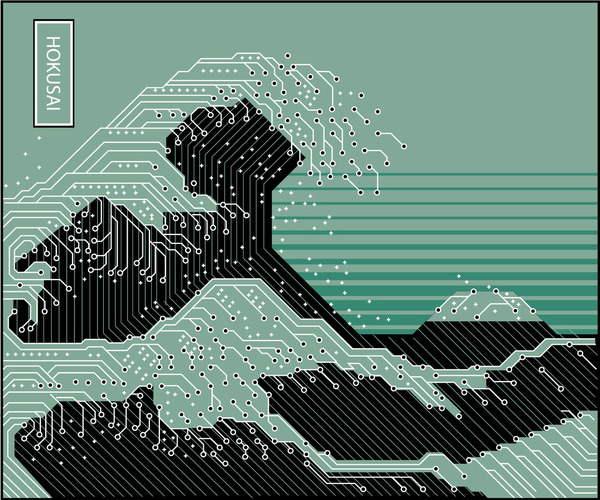
\includegraphics[width=0.9\hsize]{fig/hokusai}
\caption{Joel Betancourt znany jako Garabating - "Katsushika Hokusai Electronic Circuit Board"\label{RYS.1}}
\source{https://garabating.com/post/44549621917/katsushika-hokusai-electronic-circuit-board}
\end{figure}

Nie oznacza to jednak pełnej dowolności w projekcie, gdyż należy wziąć pod uwagę mnogość technicznej wiedzy, pomiarów i zależności takich jak: optymalizacja długości ścieżek oraz ich szerokość, ochrona miejsc narażonych na dużą temperaturę, ograniczenia mechaniczne i montażowe, itd. Nawet zastosowanie automatucznego wyznaczania ścieżek do optymalizacji nie zawsze da poprawny rezultat.\footnote{\,\href{https://www.autodesk.com/products/eagle/blog/top-10-pcb-component-placement-tips-pcb-beginner/}{Autodesk.com - Top 10 pcb component placement tips}} Z uwagi na ilość i różnorodność ograniczeń nie jest możliwa całkowita automatyzacja sprawdzania poprawności wykonanego projektu, zatem przydatna dla projektanta okazuje się wizualizacja efektu końcowego. Jest ona także niezbędnym elementem procesu marketingowego, logistycznego czy edukacyjnego. Istnieje wiele programów do projektowania PCB jednak żadne z nich, z uwagi na swoje ścisłe zastosowania, nie posiadają odpowiednich narzędzi do zaawansowanego renderowania, animacji i tworzenia szeroko pojętej “sztuki”. Popularny program do tworzenia grafiki 3D - Blender, z uwagi na możliwość rozbudowania go o dodatki jest znakomitym narzędziem mogącym wspomagać ten proces.

% ROZDZIAŁ 1


\chapter{Cel i zakres pracy magisterskiej}

Celem niniejszej pracy jest stworzenie łatwego do rozbudowania i spójnego systemu umożliwiającego import plików projektowych używanych bezpośrednio w przemyśle PCB do programu Blender, następnie interpretację i wyświetlenie pełnowymiarowego modelu 3D płytki drukowanej która powstałaby w procesie produkcji przemysłowej. Dodatek powinien posiadać prosty i przejrzysty interfejs który zapewnia dostęp do wszystkich funkcjonalności, ale nie przytłacza odbiorcy nadmiarem funkcji. Pozwoli to nie tylko osobom technicznym z poza branży grafiki komputerowej na łatwy dostęp do wizualizacji i edycji swoich projektów ale także na łatwiejszą integrację projektów przemysłowych z marketingową i graficzną częścią przemysłu.

\section{Wymagania funkcjonalne}

Zrealizowany system jest dodatkiem (ang. \emph{add-on}) do programu Blender, kompatybilnym z wersją 2.8 wzwyż. Wybór konkretnie tej wersji programu był podyktowany jego nową odsłoną oferującą między innymi nowy wygląd programu i duże zmiany w interfejsie programistycznym aplikacji (ang. \emph{API}). Wtyczka udostępnia użytkownikowi dodatkowe funkcjonalności z poziomu graficznego interfejsu programu. Następujące wymagania zostały sformułowane z punktu widzenia użytkownika.
\begin{itemize}
\item Wybranie folderu zawierającego wszystkie pliki projektu PCB lub wybranie pojedynczych plików warstw i  plików pozycji elementów (ang. \emph{"Pick And Place"})\footnote{\,Więcej o strukturze plików projektowych PCB w punkcie 1.2.3}
\item Wybranie wbudowanej lub własnej biblioteki modeli 3D
\item Wybór końcowej rozdzielczości i miejsca zapisu plików wytworzonych w procesie renderowania
\item Przycisk tworzący model 3D płytki na podstawie wybranych plików
\end{itemize}

\begin{figure}
\centering
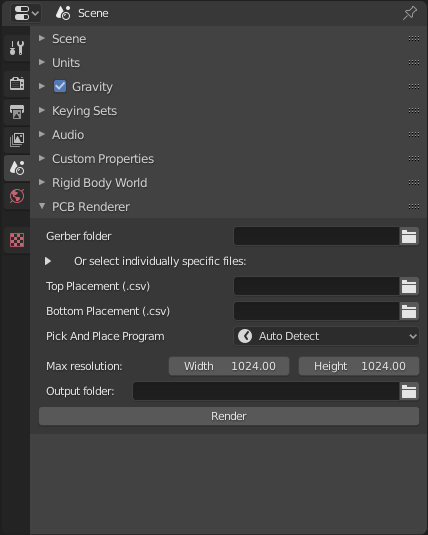
\includegraphics[width=0.75\hsize]{fig/addon_1}
\caption{Zainstalowany dodatek w programie Blender 2.82a}
\source{Opracowanie własne}
\end{figure}

\section {Opis technologii wykorzystanych w pracy}

% Python
\subsection{Python}
Python jest językiem programowania wysokiego poziomu, posiadającym aktywną społeczność i nieograniczone możliwości poprzez rozbudowę go o zewnętrzne pakiety.\footnote {\,\url{https://www.python.org/about/}} API Blendera jest w większości przygotowane do użycia właśnie Pythona i chociaż istnieją ograniczenia tego, co Python może zrobić w Blenderze, jest to jedyne oficjalnie wspierane rozwiązanie dzięki któremu wiele można osiągnąć bez konieczności zagłębiania się w kod C / C++ Blendera.

% Blender
\subsection {Blender 2.8}
Darmowy program \emph{Open-source}\footnote{\,\url{https://www.blender.org/about/license/}} cechujący się wszechstronnością i możliwością rozbudowania go o dodatkowe biblioteki lub skrypty napisane w języku Python, które rozszerzają podstawowe funkcjonalności.

Dodatek do programu Blender różni się od dodatkowej biblioteki Pythona jedynie pewnymi dodatkowymi wymaganiami jak obiekt zawierający metadane, takie jak: nazwa, wersja, kategoria, autor, etc. Określa też minimalną wersję Blendera wymaganą do uruchomienia skryptu. Dodatek jest więc sposobem na enkapsulację modułu Pythona w sposób, który użytkownik może z łatwością wykorzystać.

Blender ma wbudowany interpreter Pythona, który jest ładowany po uruchomieniu programu. Utrudnia to znacząco wykorzystanie automatycznego pobierania i instalowania zależnych od siebie pakietów, co za tym idzie, tworzony w ramach pracy system, aby ułatwić korzystanie z niego, musi być niezależny od zewnętrznych, dynamicznie pobieranych bibliotek.


\subsection{Pliki projektowe PCB}

\subsubsection {Gerber}
Nowoczesne płytki drukowane są projektowane przy pomocy dedykowanego oprogramowania a ostatnim etapem produkcji dla projektanta jest wygenerowanie między innymi plików Gerber.\cite{Khandpur}
Jest to otwarty, wektorowy, powszechnie stosowany format o standardzie ASCII, służący do przesyłania danych projektowych obwodów drukowanych do przemysłu produkcji elektroniki. Wszystkie systemy do projektowania obwodów drukowanych pozwalają na eksport projektu jako pliki Gerber i każde przemysłowe oprogramowanie do ich obróbki potrafi je interpretować, umożliwiając profesjonalistom w dziedzinie PCB bezpieczną i wydajną wymianę danych projektowych.\cite{Williams}

Płytki drukowane mogą być jednostronne (jedna warstwa miedzi), dwustronne (dwie warstwy miedzi po obu stronach warstwy podłoża) lub wielowarstwowe (zewnętrzna i wewnętrzna warstwa miedzi, naprzemiennie z warstwami podłoża).\cite{schroeder}

Pliki Gerber reprezentują między innymi warstwy miedzi, maskę lutowniczą, legendę oraz dane wiercenia i trasy. Dodatkowe atrybuty dostarczają informacji o sposobie montowania, połączeń i nazw poszczególnych elementów. Format pliku Gerber jest prosty, kompaktowy i jednoznaczny. Jest bazowany na języku \emph{G-code}, oznaczanym RS-274. Dzięki zastosowaniu 7-bitowych znaków ASCII jest czytelny dla człowieka i łatwy do debugowania. Obecnie używany od 2014 roku format to tzw. Rozszerzony Gerber (ang. \emph{Extended Gerber}) lub RS-274X.\footnote{\,\url{https://www.ucamco.com/en/gerber}}

\subsubsection {Drill}
Kolejnym, generowanym przez projektanta płytki formatem używanym w produkcji są pliki wierceń (ang. \emph{NC / CNC drill}), pierwotnie zaprojektowane przez twórców wiercących i trasujących maszyn CNC jako zastrzeżone, dedykowane formaty wejściowe dla ich urządeń. Znane są pod nazwami takimi jak: Excellon, Hitachi, Sieb \& Meyer, Posalux, itd.\cite{Charras} Wszystkie z pośród tych formatów są podobne, ponieważ opierają się na wspomnianym wcześniej G-code. Rodzaje wierceń w PCB dzielą się na otwory zwykłe - NPTH (ang. \emph{Not Plated Through Hole}) i pokryte miedzią - PTH (ang. \emph{Plated Through Hole}).\cite{voldman} Stosowanie innego standardu nie jest jednak konieczne, jako że z czasem formaty te zmieniły swoje zastosowanie i obecnie powszechnie stosowaną praktyką jest generowanie tych plików w formacie Gerber.

\subsubsection {Placement}
Ostatnim i dosyć kluczowym elementem są pliki wskazujące elementy rozmieszczane na płytce. Jest to prosty format nazywany \emph {Pick-And-Place, Placement list, X-Y file, Mount SMD}  i składa się z kilku wartości:
\begin{itemize}
\item \emph{Ref / Designator} - Indeks elementu na płytce i w projekcie
\item \emph{Value} - Wartość elementu (np. pojemność, rezystancja, napięcie)
\item Pozycja podana we współrzędnych kartezjańskich
\item \emph{Footprint / Package} - Nazwa elementu, zazwyczaj zawiera także informację o jego wymiarach
\item Rotacja elementu
\item Informacja czy objekt znajduje się na wierzchniej czy też dolnej stronie płytki
\item Ewentualne komentarze i dodatkowe informacje
\end{itemize}
Plik zawiera opis elementów montowanych za pomocą technologii montażu przewlekanego - THT (ang. \emph{Through-hole technology}) oraz powierzchniowego - SMT (ang. \emph{Surface Mount Technology}), powszechnie stosowanego przemysłowo.\cite {prasad} Nie jest to jednak format ściśle ustandaryzowany i przy masowej produkcji każdy producent musi manualnie zweryfikować opisy elementów. Na szczęście każdy program do tworzenia PCB posiada eksporter do generowania tychże plików. Dodatkowo są one proste w zapisie i z łatwością edytowalne przez człowieka.

% WRL
\subsection{Pliki VRML i X3D}
Format \emph{.wrl} zwany VRML (ang. \emph {Virtual Reality Modeling Language}) powstały w 1994 roku, stał się pierwszym internetowym formatem 3D, został później zastąpiony przez format X3D.\cite{vrml} Jego ówczesna powszechność sprawiła, że wiele programów przemysłowych tworzonych w latach dziewięćdziesiątych posiada bazy modeli w tym właśnie formacie. Więcej o praktycznym wykorzystaniu tego standardu w rozdziale \ref{bazamodeli}.

% specyfikacja formatu VRML:
% http://www.graphics.stanford.edu/courses/cs248-98-fall/Assignments/Assignment3/VRML2_Specification/

\subsection{Środowisko Visual Studio Code}
Visual Studio Code jest to darmowy edytor kodu który według badań przeprowadzanych co roku przez serwis StackOverflow\footnote{\,\url{https://insights.stackoverflow.com/survey/2018/\#development-environments-and-tools}}$^{,}$\footnote{\,\url{https://insights.stackoverflow.com/survey/2019\#development-environments-and-tools}} cieszy się coraz większym uznaniem. Wybór tego środowiska nie był jednak dyktowany jego popularnością lecz nowymi możliwościami otwierającymi się dzięki instalowaniu w nim rozszerzeń.\footnote{\,\url{https://code.visualstudio.com/docs/editor/extension-gallery}} Dodatek stworzony przez Jacques Lucke na potrzeby rozwoju addonów do programu Blender pozwala między innymi na automatyzację procesu aktualizowania tworzonego addonu przez tworzenie skrótu w wewnętrznych folderach Blendera, co znacznie przyśpiesza pracę nad systemem. Ponadto posiada ułatwienia takie jak debugowanie w konsoli, tworzenie odpowiednich struktur i przydatne komendy. Sposób działania dodatku ma na celu także upewnienie się, że rozszerzenie nie koliduje z innym menedżerem pakietów Pythona.\footnote{\,\url{https://marketplace.visualstudio.com/items?itemName=JacquesLucke.blender-development}} 


% Czy i gdzie to dać?
% przegląd krytyczny literatury - analiza krytyczna dotychczasowych badań/rozwiązań z zakresu tematu?
% majenkotech i Eagle2Blender oba bardzo specyficzne do gEDA i Eagle nieposiadające interfejsu, niewygodne do użycia, wymagają dotatkowych narzędzi, znikoma dokumentacja
%https://bitbucket.org/hyOzd/pcb2blender/src/master/
% https://github.com/majenkotech/PCB-Blend

\chapter{Architektura zrealizowanego systemu}
Aby zobrazować podstawowe założenia projektu, w niniejszym rozdziale zostanie omówiona koncepcyjna struktura zrealizowanego systemu. Przedstawi ona bardziej szczegółowo mechanizmy działania najważniejszych komponentów aplikacji, a finalnie pomoże w samym procesie tworzenia oprogramowania.

\section{Założenia i wymagania projektowe}
W przypadku tak rozległych możliwości rozwoju systemu, kluczowe jest właściwe zdefiniowanie wymagań projektu i dążenie do ich realizacji. Postawienie ograniczeń w kwestii wspieranych formatów na jakich działał będzie dodatek jest konieczne z uwagi na zróżnicowanie technologii używanych w procesie tworzenia PCB. Z drugiej strony nacisk na modułowość rozwiązania pozwoli później na łatwiejsze dodanie dowolnego rozszerzenia.
System powinien implementować wszystkie następujące funkcjonalności:

\begin{itemize}

\item Implementacja interfejsu przy pomocy API Blendera 2.8

\item Czytanie i interpretacja plików Gerber (RS-274X)

\item Tworzenie modelu płytki na podstawie otrzymanych plików, zgodnego z rzeczywistymi wymiarami

\item Czytanie i interpretacja pliku placement w formacie .csv

\item Udostępnienie użytkownikowi możliwości użycia dostarczonej lub własnej bazy modeli podzespołów

\end{itemize}

\section {Struktura projektu}
Podstawowy wybór strukturalny następującego rozwiązania jest podyktowany wymaganiami i sposobem komunikacji z API Blendera. Struktura folderów dodatku do programu Blender jest dowolna z założeniem, że w folderze głównym znajduje się plik \emph{\_\_init\_\_.py} odpowiedzialny za rejestrowanie dodatku. Jest on automatycznie wykonywany po wybraniu folderu i włączeniu addonu w sekcji "Dodatki" w programie Blender. Pozostałe elementy są pogrupowane według konwencji modułów w języku Python, zatem każdy moduł posiada swój folder, jest to jednak podyktowane tylko enkapsulacją modułów i wygodą w używaniu referencji między skryptami.

\subsection{Główna struktura interfejsu API Blendera}
Z poziomu kodu, API Blendera udostępnia główne moduły pod słowem kluczowym \textbf{bpy}\footnote{\,\url{https://docs.blender.org/api/current/index.html}} a jego podstawowe i główne elementy to:
\begin{itemize}
\item \textbf{bpy.data} -- Zapewnia dostęp do danych bieżącego pliku \emph{*.blend} (Jest to rozszerzenie używane przez program Blender). Każde z jego pól jest zbiorem obiektów danego typu (sceny, obiekty, zbiory wierzchołków, materiały, kolekcje itp.).
\item \textbf{bpy.context} -- Zawiera wszelkie dane środowiskowe obrazujące bieżący stan programu (bieżący wybór, tryb i region edytora) oraz wiele globalnych właściwości.
\item \textbf{bpy.ops} -- Zawiera wszystkie \emph{Operatory} Blendera. (W API każda komenda Blendera jest zaimplementowana jako metoda klasy \emph{Operator}).
\item \textbf{bpy.types} -- Posiada definicje wszystkich klas używanych w strukturach.
\end{itemize}
Istnieje także wiele mniejszych, pobocznych modułów i podmodułów pomocniczych. Niektóre z nich nie należą nawet do głównego modułu \textbf{bpy}. Mniejsze moduły, między innymi: bpy.props, bpy\_extras, bpy.utils, mathutils, bmesh, będą omówione w dalszej części tej pracy.
% ew. zostaną wspomniane w rozdziale X odnośnie implementacji

\subsection{Implementacja wzorca projektowego} \label{mvp}
MVP (ang. \emph{Model–view–presenter}) jest wzorcem architektury oprogramowania opierającym się na trzech głównych założeniach:\cite{mvp}
\begin{itemize}
\item Model reprezentuje dane które są przetwarzane i wysyłane do prezentera
\item Widok (\emph{View}) wyświetla dane uzyskane z prezentera i przekazuje dane wejściowe wprowadzane przez użytkownika do prezentera
\item Prezenter jest wywoływany z Widoku aby wyświetlać dane pobrane z Modelu i przetwarzać dane wejściowe
\end{itemize}
System został zaimplementowany w oparciu o ten właśnie wzorzec z uwagi na to, że jest to struktura logicznie wynikająca ze sposobu używania API Blendera.
W tym przypadku, w dużym uproszczeniu Modelem jest logika modułu, Widokiem -- klasa odpowiedzialna za renderowanie i odbieranie danych wejściowych a Prezenter to API Blendera.
\newline


Skrypty w języku Python można zintegrować z Blenderem na następujące sposoby:
\begin{itemize}
\item Definiując silnik renderujący.
\item Poprzez zdefiniowanie operatorów.
\item Poprzez zdefiniowanie menu, nagłówków i paneli.
\item Wstawiając nowe przyciski do istniejących menu, nagłówków i paneli.
\end{itemize}
W Pythonie odbywa się to poprzez zdefiniowanie klasy, która jest podklasą istniejącego typu. 
Tak więc, przechodząc do rzeczywistego stanu rzeczy, omawiany addon o nazwie \emph{PCB-Blender} jest zdefiniowany jako skompresowane archiwum składające się z następujących elementów:
\begin{itemize}
\item \emph{PCB\_LayoutPanel} -- Klasa odpowiedzialna za wyświetlanie interfejsu i przekazywanie danych wybranych przez użytkownika, dziedzicząca z klas abstrakcyjnych \emph{Panel} i \emph{ImportHelper}. Wraz z klasami pomocniczymi znajduje się w pliku PCB\_Blender\_panel.py,
\item \emph{PCB\_Generate} -- Klasa dziedzicząca z klasy \emph{Operator}, znajdująca się razem z klasami pośrednimi w pliku PCB\_Blender.py,
\item \emph{\_\_init\_\_.py} -- Plik zawierający metadane i rejestrujący powyższe klasy,
\item Foldery zawierające pozostałe moduły Pythona do których odnosi się główny Operator -- \emph{PCB\_Generate}.
\end{itemize}

\subsection{Baza modeli} \label{bazamodeli}

Jednym z pierwszych z wyzwań podczas tworzenia dodatku był dobór zasobów w postaci modeli 3D. Aby zrealizować założenia pracy, wymagana była baza modeli podzespołów elektronicznych montowanych na PCB. Z uwagi na mnogość producentów, rodzajów i typów podzespołów oraz fakt, że każdy program służący do projektowania może oznaczać je inaczej, optymalnym rozwiązaniem wydaje się udostępnienie użytkownikowi podstawowej bazy modeli. Ponadto zastosowanie szukania modeli częściowo dopasowanych nazwą. Z uwagi na fakt, że niemożliwym jest obsługa wszystkich wyjątków, koniecznością staje się umożliwienie użytkownikowi kożystanie z własnych, wybranych modeli. Istnieje wiele stron udostępniających modele 3D na zasadach komercyjnych jak i darmowych licencji. Są one często wykorzystywane przez twórców jak i programy projektowe. Oto kilka z nich zaprezentowanych w tabeli: \ref{fig:table}.

\begin{table}[htb]
\begin{tabular}{|l|l|l|} \hline
Adres URL \\ \hline
\url{https://grabcad.com/} \\ \hline
\url{https://www.3dcontentcentral.com/} \\ \hline
\url{https://www.digikey.com/en/resources/3d-models} \\ \hline
\url{https://www.te.com/} \\ \hline
\url{https://www.traceparts.com/en} \\ \hline
\end{tabular}
\caption{Publicznie dostępne bazy modeli podzespołów}
\source{Opracowanie własne}
\label{fig:table}
\end{table}
Nie posiadają one jednak możliwości masowego pobierania modeli. Pomijając tą niedogodność, która musiałaby być rozwiązana skryptem automatyzującym pracę, również ilość pobranych materiałów znacznie przekroczyłaby racjonalny poziom. Z pomocą przychodzi tu darmowy zbiór modeli używanych w programie KiCad\footnote{\,\url{https://kicad.github.io/packages3d/}}. Modele są dostępne między innymi w formacie \emph{*.wrl} więc można zaimportować je do Blendera. Więcej o przetwarzaniu plików \emph{*.wrl} oraz tworzeniu bazy modeli w rozdziale \ref{wrl}.



\chapter{Szczegóły implementacyjne systemu}
W tym rozdziale zostanie omówiony sposób implementacji kluczowych i pobocznych funkcjonalności systemu.
\section {Rejestrowanie addonu}
Każdy dodatek do Blendera musi posiadać obiekt \emph{bl\_info}, zawierający metadane addonu oraz implementować metody \emph{register()} oraz \emph{unregister()}. Wprowadzone w wersji 2.8 API usprawnienia znacznie ułatwiają ten proces. Jeżeli nie potrzebujemy dodatkowych funkcjonalności podczas rejestrowania i usuwania dodatku lub jego komponentów, możemy użyć funkcji \emph{register\_classes\_factory} z pakietu \textbf{bpy.utils}, która automatycznie je zaimplementuje.

\lstset{caption={\emph{\_\_init\_\_.py} -- Plik rejestrujący dodatek.}}
\begin{lstlisting}
bl_info = {
	"name" : "PCB-Blender",
	"author" : "Adam Makiewicz",
	"description" : "Addon for generating models of PCB from Gerber files",
	"blender" : (2, 80, 0),
	"version" : (0, 1, 4),
	"category" : "Generic",
	"location" : "Scene Properties > PCB Renderer"
}
	import bpy
	from . PCB_Blender_panel import PCB_LayoutPanel
	from . PCB_Blender import PCB_Generate

	classes = (PCB_LayoutPanel, PCB_Generate)
	register, unregister = bpy.utils.register_classes_factory(classes)
\end{lstlisting}

\section {Implementacja interfejsu}

Klasa \emph{PCB\_LayoutPanel} dostarcza całą funkcjonalność renderowania interfejsu dzięki dziedziczeniu z wewnętrznej klasy bazowej \emph{Panel}. Właściwości takie jak nazwa, miejsce wyświetlania się panelu, wielkość, kontekst, typ regionu itp. muszą być zdefiniowane w odpowiednim formacie. Dzięki temu są one automatycznie interpretowane przez API i poprawnie wyświetlane. Właściwości klasy zaczynają się od przedrostka \emph{bl\_}, jest to konwencja używana do odróżnienia wbudowanych właściwości klas Blendera od tych, które zostają dodane przez programistę.

\lstset{caption={Przykład właściwości panelu z pliku \emph{PCB\_Blender\_panel.py}}}
\begin{lstlisting}
class PCB_LayoutPanel(Panel):
	bl_label = "PCB Renderer"
	bl_idname = "SCENE_PT_layout"
	bl_space_type = 'PROPERTIES'
	bl_region_type = 'WINDOW'
	bl_context = "scene"
\end{lstlisting}

\vspace{5mm}

Oprócz posiadania statycznych właściwości, klasa powinna przechowywać i przekazywać dynamiczne zmienne. Aby dodać zmienną do zarejestrowanej klasy w Blenderze należy użyć jednej z Definicji Właściwości (ang. \emph{Property Definition}) z modułu \textbf{bpy.props}. Moduł ten definiuje właściwości rozszerzające wewnętrzne dane Blendera. Wynik tych funkcji służy do przypisywania właściwości do klas zarejestrowanych w Blenderze i nie można ich używać bezpośrednio. Są to między innymi \emph{StringProperty, FloatProperty, EnumProperty, BoolProperty} lub dowolne ich zestawienie jako jedna strukturalna zmienna. Funkcje wymagają każdorazowego zdefiniowania nazwy, opisu, wartości domyślnej, podtypu itp. więc aby uniknąć redundancji kodu zostały stworzone funkcje pomocnicze, przedstawione we fragmencie kodu \ref{Listing3}. Zdefiniowanie typu \emph{StringProperty} jako ścieżka do pliku lub folderu sprawia, że do elementu wyświetlającego tą zmienną automatycznie zostanie przypisany przycisk otwierający eksplorator plików w celu wybrania pliku.

% trzeba chyba dopisać coś do powyższego fragmentu, albo dać \newpage bo fragment kodu przechodzi przez 2 strony...
\newpage

\lstset{caption={Funkcje pomocnicze tworzące zmienną o tym samym typie lecz innym zastosowaniu -- ścieżki pliku i ścieżka folderu}\label{Listing3}}
\begin{lstlisting}
def FilePath(_name, _description="", _default=""):
	return StringProperty(name=_name, default = _default,
	description=_description, subtype = 'FILE_PATH')
    
def DirPath(_name, _description="", _default=""):
	return StringProperty(name=_name, default = _default,
	description=_description, subtype = 'DIR_PATH')
\end{lstlisting}

Oprócz zmiennych, aby poprawnie zaimplementować dany interfejs, klasa musi zawierać też funkcję \emph{draw()} odpowiedzialną za renderowanie elementów w panelu. Wygląd i rozmieszczenie elementów jest zdefioniowane przy pomocy obiektu klasy \emph{UILayout} i jego elementów takich jak kolumny i rzędy w których umieszcza się referencje do wspomnianych wyżej, dynamicznych zmiennych. Następnie w jednym z elementów zostaje umieszczone wywołanie operatora z klasy \emph{PCB\_Generate}, który przyjmuje kontekst w którym zostal wywołany --- a zatem również wszystkie zmienne.

% mogę to bardziej rozpisać i dać przykłady, ale są to bardzo proste i trywialne jednolinijkowce. Ewentualnie jeszcze logika chowania się kilku elementów, jakieś 3 linijki kodu

\section {Interpretacja plików Gerber  (excellon + renderowanie kolejny punkt)}
Jak wspomniano wcześniej, funkcja wykonania operatora (\emph{execute}), pobiera w argumencie informacje o środowisku wywoływanego i bieżący kontekst.
API Blendera wymaga od klasy operatora implementacji ściśle zdefiniowanych metod. Jest to rodzaj „umowy” pomiędzy skryptem a systemem rdzenia Blendera. Zgadzamy się na wdrożenie wymaganych funkcji w swojej klasie. Blender zgadza się wywoływać je w ściśle określonych okolicznościach. W programowaniu obiektowym taka lista zakontraktowanych funkcji i właściwości nazywa się „interfejsem”. Aby trochę pomóc w jego implementacji, Blender API dostarcza klasę bazową dla operatorów pochodnych, o nazwie \emph{bpy.types.Operator}. W żargonie programowania obiektowego Operator jest tak zwaną „klasą abstrakcyjną”. Po prostu zapewnia domyślne, puste implementacje wszystkich metod wymaganych przez interfejs. Nasza klasa operatora dziedziczy tę domyślną treść z klasy bazowej.

% moduły zewnętrzne pythona: cairo, gerber etc.
%interpretacja Gerber (RS-274X) i Excellon, interpretacja kształtów i rysowanie za pomoca krzywych, renderowanie obrazu płytki
%PCB Tools currently supports the following file formats:
%    Gerber (RS-274X)
%    Excellon
%with planned support for IPC-2581, ODB++ and more.
%https://pcb-tools.readthedocs.io/en/latest/about.html
% gdzie zamieścić info o licencji?

% podział na funkcje użytkowe, tworzące siatkę, renderujące
% brakujące pliki nie powinny psuć procesu
% możliwość wybrania dowolnie wielu lub sprecyzowanie konkretnych plików
% konwersja z mil/mm
% renderowanie modelu z wymiarów warstwy outline/jakiejkolwiek innej warstwy jeżeli nie ma w przypadku nie podania outline'a
% wymiary, shader, przesuwanie, idk
\section {zanim będziemy mogli wczytać plik placement musmy mieć modele - stworzenie bazy modeli, importer *.wrl\label{wrl}}

% przejrzeć commity i wypisać funkcjonalności zaimplementowane w importerze

% tworzenie bazy modeli - importer *.wrl
% https://kicad.github.io/packages3d/
% działanie w przypadku braku modeli
% niedziałający importer w Blenderze przy implementacji w rozdziale 2
% musi w miarę mało ważyć więc baza modeli będzie osobno
%All Parts in this repository are licensed under CC-BY 3.0 http://creativecommons.org/licenses/by/3.0/
% gdzie zamieścić info o licencji?
\section {czytanie placement .csv i stawianie modelu}


% ew .Funkcjonalność panelu

%(placement files) ładowanie komponentów i linkowanie plików pomysł wzięty z: https://github.com/majenkotech/PCB-Blend
% obsługa powtarzających się elementów (cache)
%  smart search - w przypadku nie znalezienia - w przypadku nie znalezienia w ogóle - pusty (może możliwość wyłączenia tego? ale po co jak można usunąć model po prostu...)
\chapter{Podsumowanie}

    % przypomniec cel pracy,
    % jak zostały spełnione wymagania: implikacje, konsekwencje, walory,
    % w jaki sposób zaimplementowana technologia rozwiązuje postawione problemy
    % czy wszystkie problemy zostały rozwiązane,
    % jakie nie zostały rozwiązane, dlaczego?

W efekcie końcowym zostały utworzone \emph{de facto} 2 addony.
%Aplikacja,  mimo  iż  jest  dedykowana  dla  projektów stworzonych w gEDA, KiCad,  jest  o  wiele  bardziej uniwersalna, ponieważ w praktyce wystarczy dodać modele, aby uzyskać format możliwy do odczytania. Podsumowując,  w  wyniku  prac  implementacyjnych  udało  się  zrealizować projekt,  który  jest  zgodny  z  przyjętymi  wcześniej  wymaganiami  i  założeniami przedstawionymi  na  etapie  opracowywania  koncepcji  rozwiązania.  Pomijając  jedną dużą modyfikację związaną ze zmianą metodologii postępowania, projekt powstałych klas pozostał w niezmienionej formie. Warto także zaznaczyć, że przyjęta architektura realizuje   wszystkie   postawione   wymagania   funkcjonalne.   Niestety   aplikacja   nie uniknęła wad. Jedną, ale za to dość poważną, jest spore zapotrzebowanie na pamięć przy przetwarzaniu dużych plików. Jednak dla mniejszych zbiorów danych wydajność czasowa jest na akceptowalnym poziomie. W  kolejnym  rozdziale  przedstawione  zostanie  podsumowanie całokształtu prac związanych z analizą oraz implementacją omawianej aplikacji.

\section{Realizacja założonych celów pracy magisterskiej}
\section {Problemy napotkane podczas realizacji systemu}
\subsection {importer *.wrl}
\section{Możliwości rozwoju systemu}
% globalne definiowane kolorów modelu?
% style PCB w gerber.cairo
% wspieranie innych rozszerzeń:
https://pcb-tools.readthedocs.io/en/latest/about.html
(with planned support for IPC-2581, ODB++ and more.)

\section{Wnioski}



% zakończenie
\summary
%Możliwości, jakie stoją przed archiwum prac magisterskich opartych na XML-u, są ograniczone jedynie czasem, jaki należy poświęcić na pełną implementację systemu. Nie ma przeszkód technologicznych do stworzenia co najmniej równie doskonałego repozytorium, jak ma to miejsce w przypadku ETD. Jeżeli chcemy w pełni uczestniczyć w rozwoju nowej ery informacji, musimy szczególną uwagę przykładać do odpowiedniej klasyfikacji i archiwizacji danych. Sądzę, że język XML znacznie to upraszcza.

% załączniki (opcjonalnie):
%\appendix
%\chapter{Tytuł załącznika 1}
%Treść załącznika 1.


% literatura (obowiązkowo):
\bibliographystyle{unsrt}
\bibliography{literatura}

% spis tabel (jeżeli jest potrzebny):
\listoftables

% spis rysunków (jeżeli jest potrzebny):
\listoffigures

\oswiadczenie

\end{document}
